\documentclass[12pt]{article}
\usepackage{graphicx}
\usepackage{float}

\topmargin 0.0cm
\oddsidemargin 0.2cm
\textwidth 16cm 
\textheight 21cm
\footskip 1.0cm

\title{Final}
\author{Zach Stecher}
\date{Due: 12/16/16}

\begin{document}

\maketitle

\section*{1) Support Vector Machines: Run the provided program for 1,000 samples and discuss hyperparameter results. Repeat for 10,000 samples.}

I performed this experiment multiple times for each sample number. From looking at the results, it appears the parameters $\textit{C}$ and $\gamma$ are inversely tied together. At the beginning of each run, $\textit{C}$ would generally start small, while $\gamma$ would start high. Both parameters would end up converging on nearly the same score every run, though. $\textit{C}$ would normally end up starting around 0.03125 and ending around 0.5, while $\gamma$ would end up starting around 3.05 and always end at 2.0. Because $\textit{C}$ refers to the cost of misclassification (I.E. the penalty for a misclassified point) and $\epsilon$ refers to the zone of insensitivity (I.E. what makes the SVM ``good enough'' to stop optimizing) we can normally expect the two to be somewhat tied together in order to achieve the best score. A lower $\textit{C}$ constitues a ``soft margin'', allowing a higher number of misclassified points in exchange for a smoother hyperplane and less overfitting. In the same vein, a lower $\epsilon$ means a lower zone of insensitivty surrounding the proposed hyperplane, resulting in a stricter machine where more answers are considered incorrect, thus resulting in a higher overall penalty.

\begin{figure}[H]
\raggedright
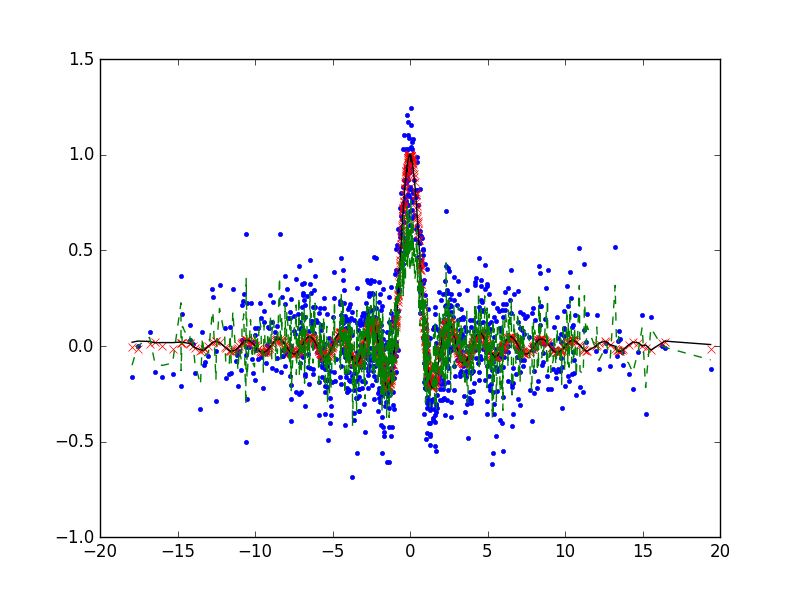
\includegraphics[width=1\textwidth]{SVMsincN10000.png}
\caption{N = 10,000}
\end{figure}

\section*{2) Run the provided program and save the plotted results. Discuss the results and the hyperparameters.}

\begin{figure}[H]
\raggedright
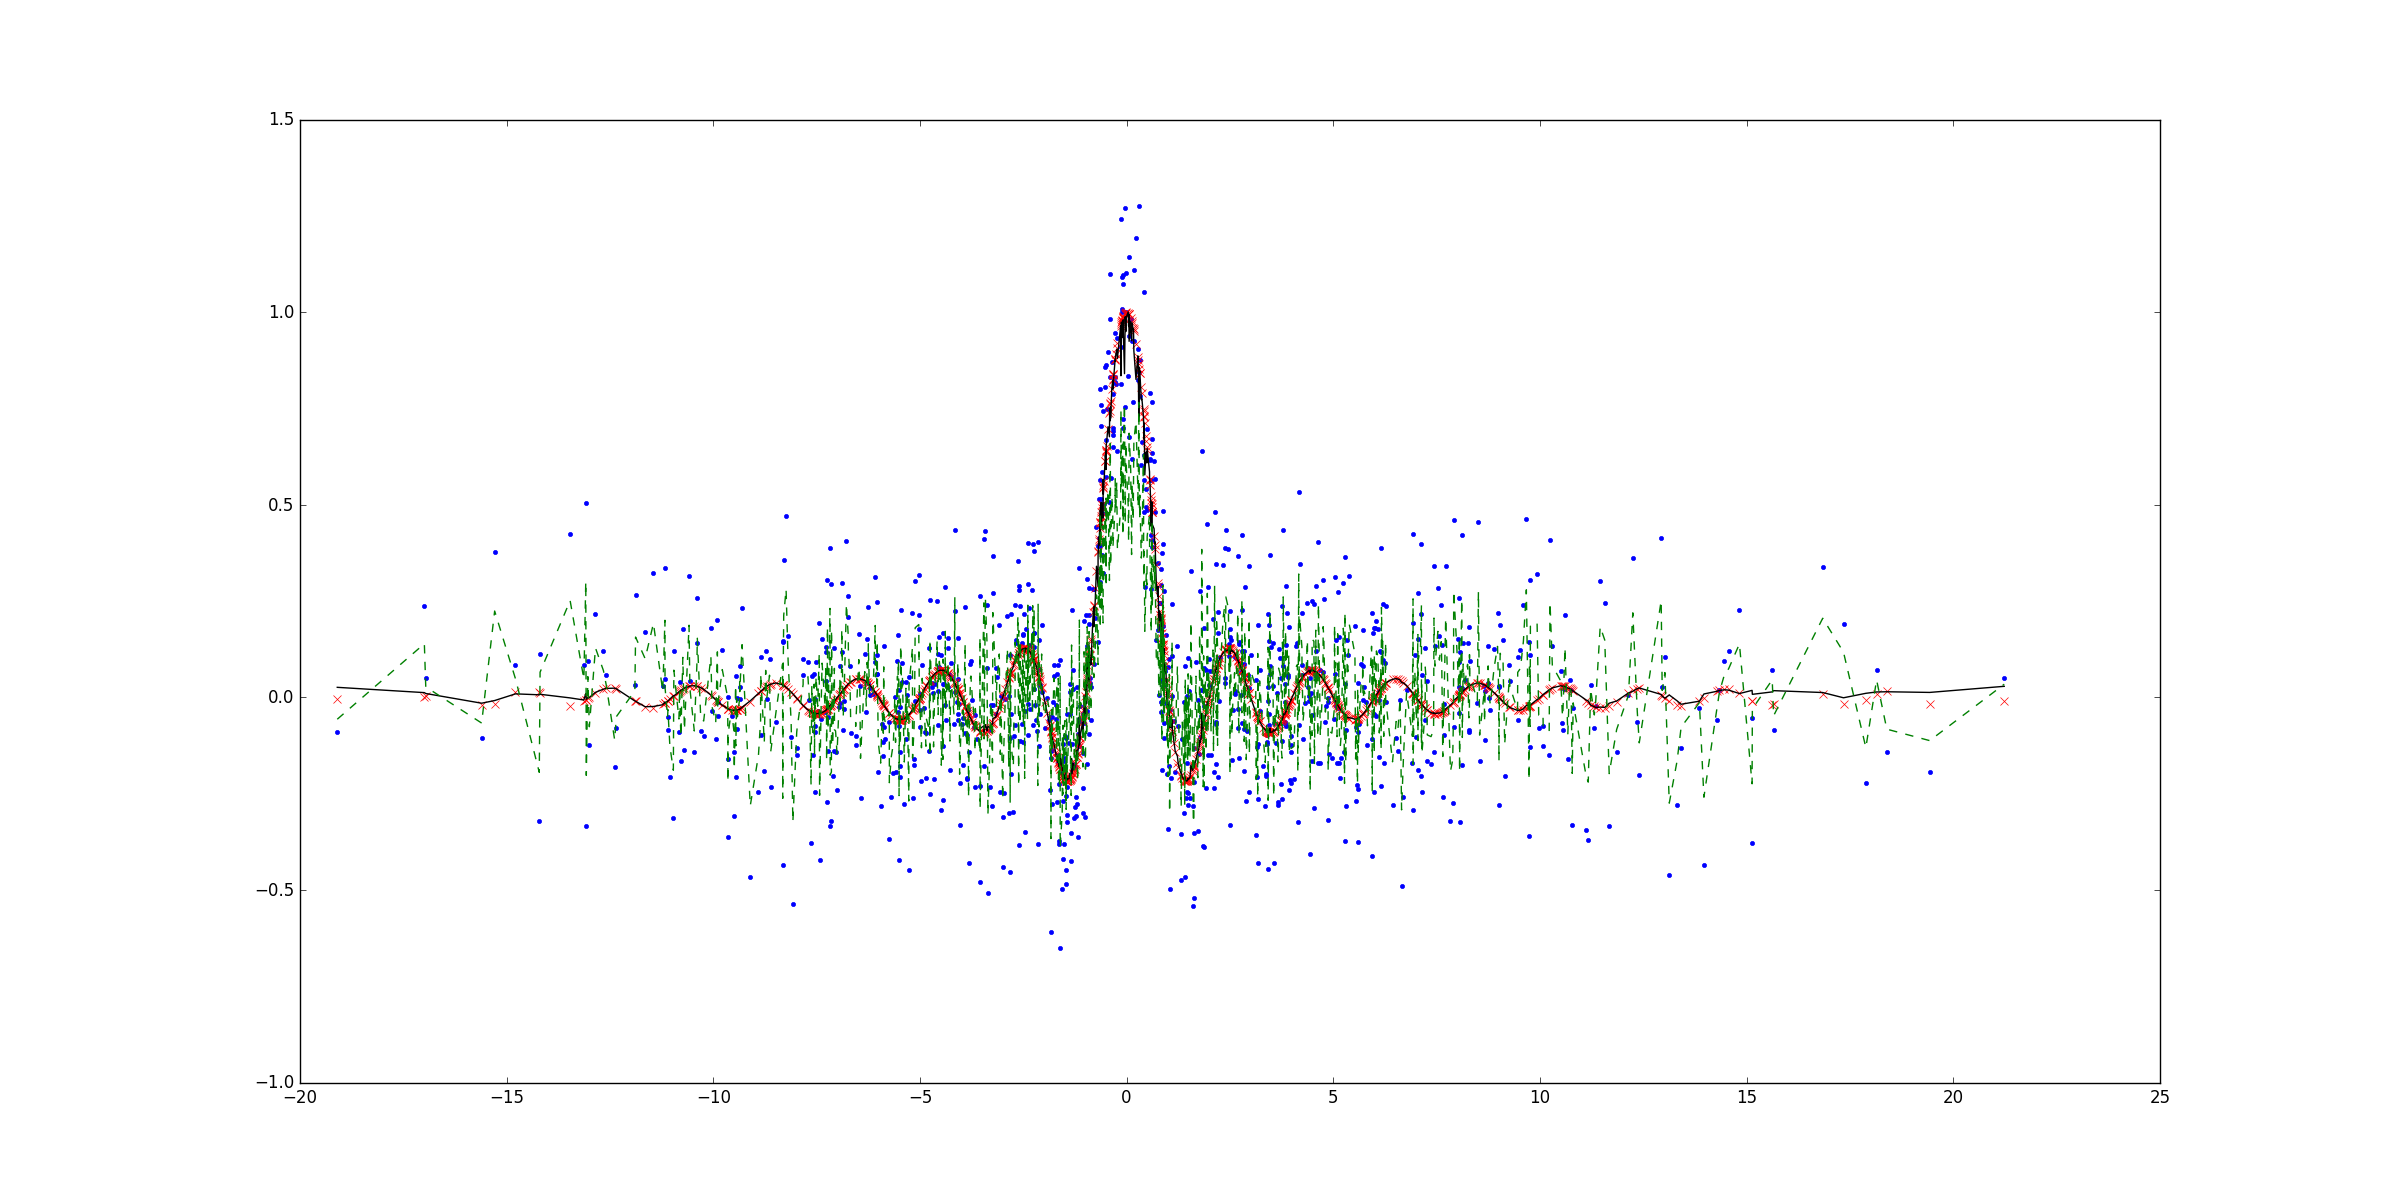
\includegraphics[width=1\textwidth]{SVMdig.png}
\caption{SVM Dig}
\end{figure}

\begin{figure}[H]
\raggedright
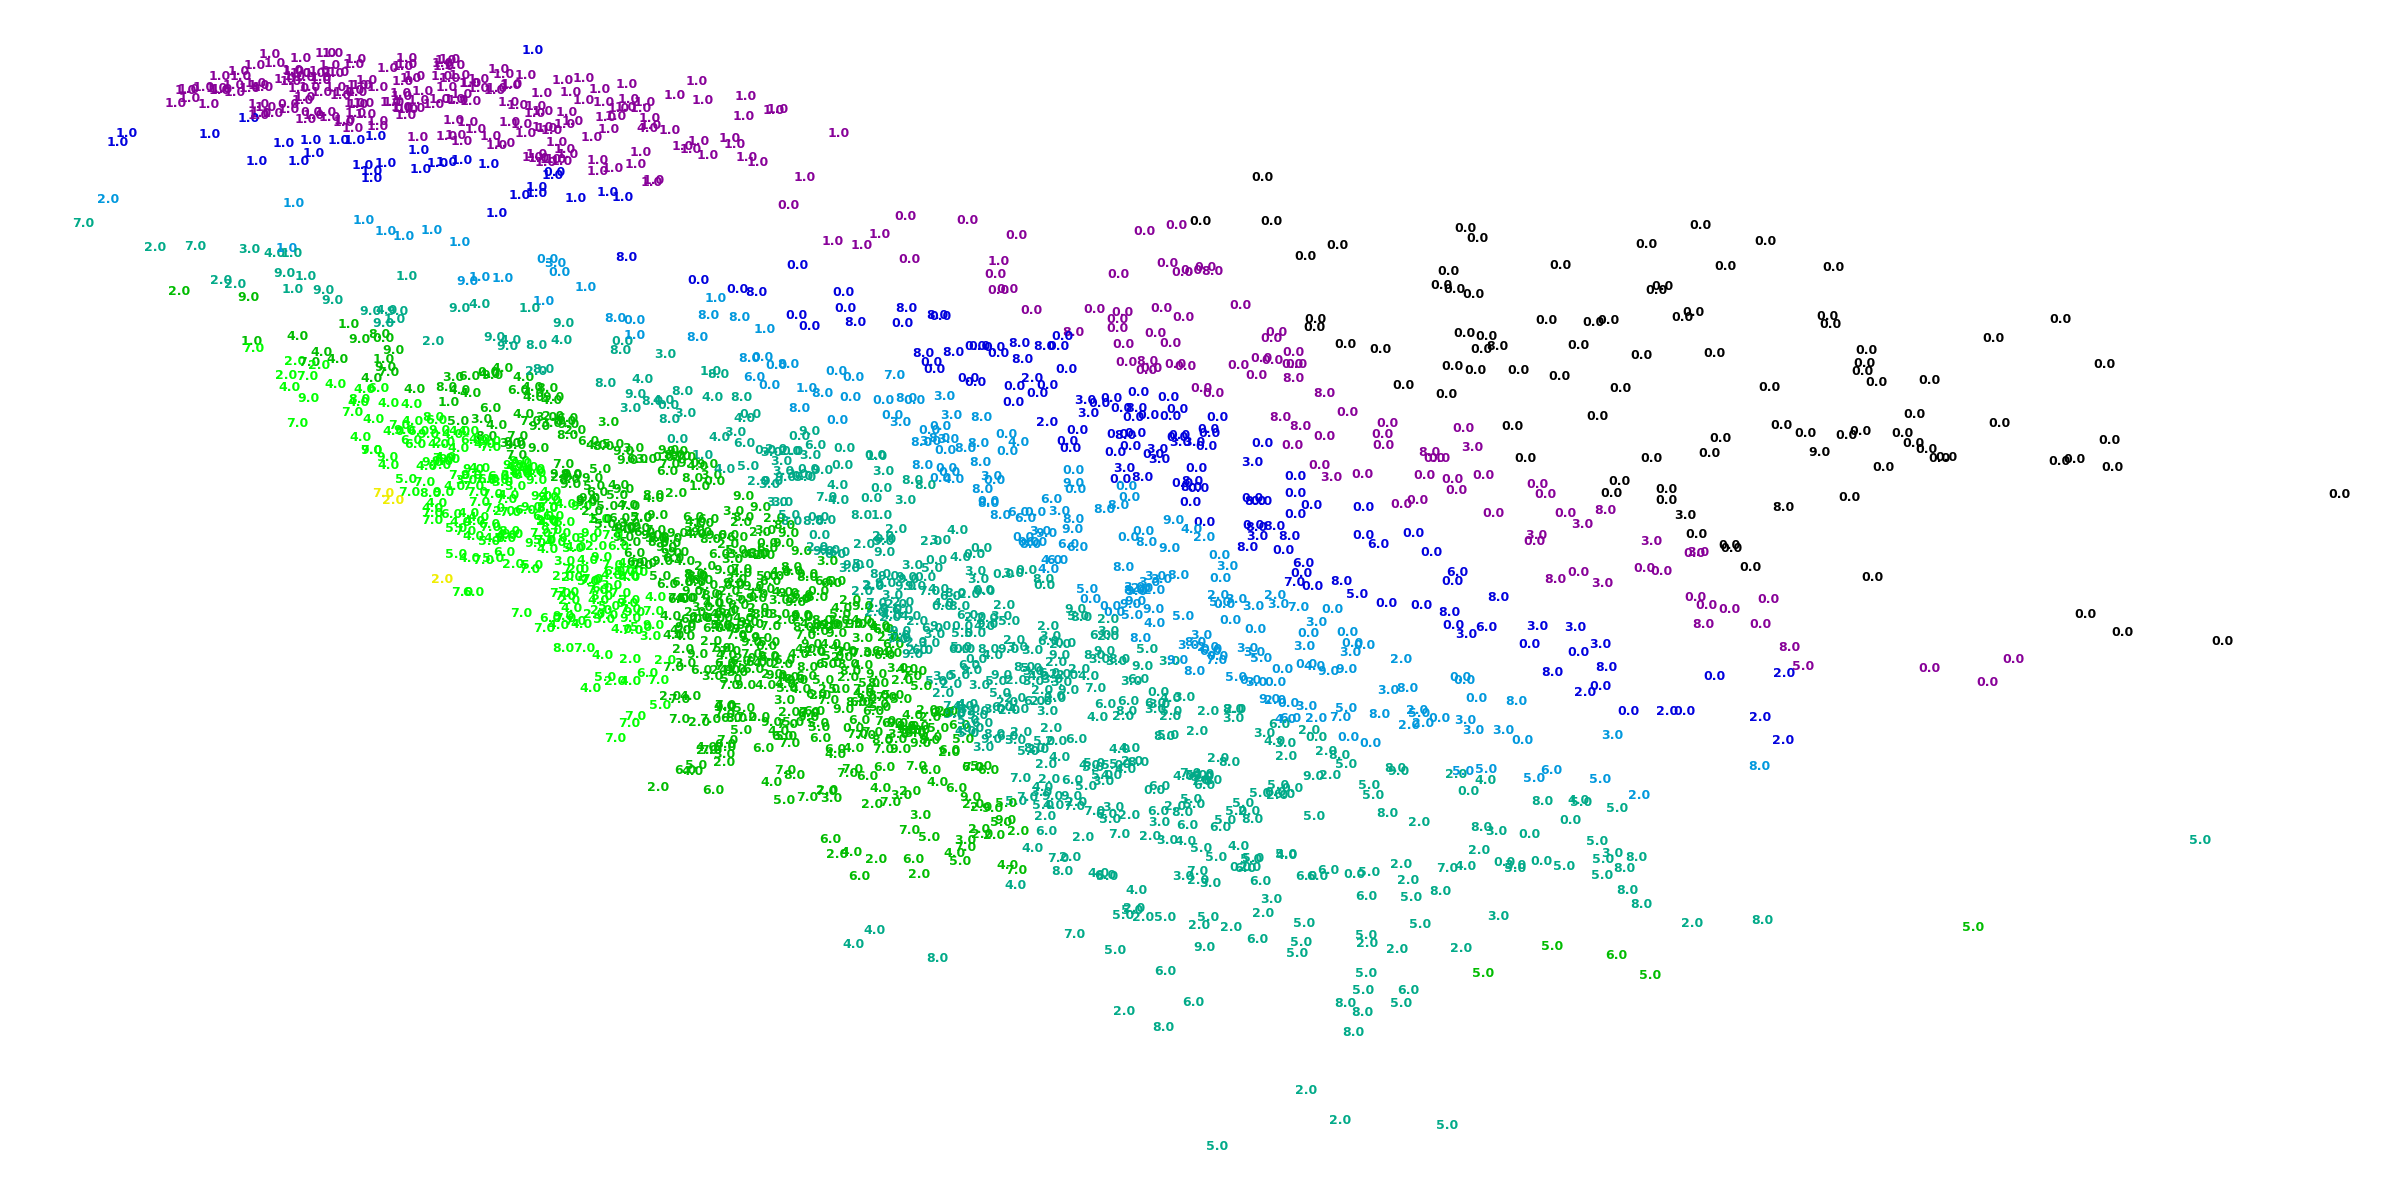
\includegraphics[width=1\textwidth]{SVMdigSpread.png}
\caption{SVM Data Plot}
\end{figure}

Looking at the plot it's clear this data was not linearly seperable. It's obvious that a lot of mistaked were tolerated in pursuit of generalization of the model. This is correlated by the final hyperparameter score of $\textit{C} = 4096.0$, $\epsilon = 1.6$, $\gamma = 0.03125$, with a final training set score of 0.347172 and a final testing set score of 0.329697. While mistakes were heavily penalized according to the high $\textit{c}$ value, the middling $\epsilon$ value considered data points that were close to the target (in terms of features) as correct, resulting in some misclassifications that were not recognized by the model as misclassifications. It also seemed that the higher the value of $\textit{C}$, the higher the value of $\epsilon$ needed to be in order to result in a better CV score. This is likely because the harsher the misclassification penalty in a non-linearly seperable dataset, the more forgiving the model needs to be in order to find a solution that works and doesn't suffer from overfitting.

\end{document}